\chapter{Asking Millionaires How They Got Rich (Dallas)}

This lecture proceeds by encounter rather than by formal theorem. We are taken through Highland Park in Dallas, shown a series of operators, executives, athletes, and owners, and asked to extract from each of them a small piece of the machinery of wealth. If we slow the lecture down and preserve its order, the structure becomes clear. First we are shown scale. Then we are shown what actually governs scale: customer knowledge, culture, discipline, exits, delegation, concentration, liquidity, and finally the proposition that the most durable route upward is to make other capable people more successful.

\section{Dallas as a Field Test for Wealth}

The lecture begins with a cold open of cars, titles, and large numbers. This is not yet the argument. It is the bait. The argument begins only when the host tells us where we are and what we are doing: we are in Highland Park, we are sampling visible wealth in the street, and we are going to ask the same basic question repeatedly, namely how success was built.

What the cold open contributes is a ledger of scale. These quantities do not belong to one person or one company; they are the scattered numerical markers that the lecture will later organize into cases.

\begin{align}
I_{\mathrm{athlete}} &\approx \$11\text{ million},\\
R_{\mathrm{business}} &\approx \$60\text{ million},\\
V_{\mathrm{ops}} &\approx \$700\text{ million},\\
V_{\mathrm{exit}} &\in \{\$365\text{ million},\ \$3.5\text{ billion}\}.
\end{align}

We also get a later footprint claim from the tanning-franchise owner, which functions as a simple operating measure of geographic scale:

\begin{equation}
N_{\mathrm{loc}} \ge 75,\qquad N_{\mathrm{states}} = 13.
\end{equation}

These are not yet organized into a single model. The lecture uses them first as evidence that Dallas is populated by people who have actually run large systems, and only afterwards starts to ask what those systems have in common.

\section{Consumer Obsession and Character at Scale}

The first full doctrinal statement comes from the Frito-Lay CEO. The lecture begins by surprising itself: an ordinary street interaction suddenly becomes a conversation with the head of a multi-billion-dollar consumer-products company. Once that surprise is registered, the host asks the right question: how does one build something on that scale?

The answer is deliberately double. On the one hand there is a founding myth: Herman Lay selling potato chips from a truck, working hard, taking care of customers, taking care of employees. On the other hand there is a modern operating rule: in a large consumer business one must understand the consumer better than anyone else and use technology to keep up with what the consumer wants now.

Schematically, the lecture compresses this into an operating doctrine of the form

\begin{equation}
\text{consumer understanding} + \text{technology} + \text{hustle} + \text{authenticity}
\longrightarrow
\text{scalable business}.
\end{equation}

We should not mistake the notation for a quantitative model. It is a way of preserving the order in which the speaker motivates the pieces. First comes the founder story, because the lecture wants to keep the possibility of ascent open. Then comes the correction: in the present environment one does not scale by myth alone, but by disciplined attention to what the customer is doing.

When the host asks what actually enabled this rise to chief executive rank, the answer again refuses a single heroic variable. Preparation matters. Luck matters. Being in the right place at the right time matters. But the moral correction comes immediately: one may work hard and still fail if one is a jerk. The lecture is already moving away from a purely competitive picture toward a social one.

\section{The Company Is Not the CEO}

The next interview changes the emphasis. We move from consumer-products scale to retail turnaround leadership, and the first major thesis is almost anti-heroic: the company is not made successful by the CEO alone. The people who work in the company make the success, and the CEO's responsibility is to make them realize how important they are.

That claim immediately deepens into a second one. There is no universal formula imported from the leader's personality. Each company has its own culture, and the executive must understand who the company is, not simply impose who he is. Culture is not decoration here; it is prior information.

The lecture then arranges the management problem in a causal order. Even if one grants that the shareholder stands at the top of the formal hierarchy, the practical path to shareholder welfare runs through customers and employees.

\begin{equation}
\text{customer care} + \text{employee care}
\longrightarrow
\text{shareholder protection}.
\end{equation}

This is a strong and useful reversal. The shareholder may be able to fire management, but the lecture insists that the shareholder cannot be served directly if the customer is neglected.

\subsection{Question \& Answer}

\paragraph{Question.} If shareholders formally come first, what should management actually put first in practice?

\paragraph{Answer.} The lecture's answer is operational rather than ideological. We first understand the culture of the firm. We then understand the customer. We make sure the people inside the company are taken care of. Only through that chain do we arrive at shareholder value. The order of causation is not the same as the order of legal power.

This is one of the cleanest conceptual turns in the lecture, and it deserves to remain explicit. Without it, the section would collapse into generic advice. With it, we keep the tension: formal primacy on one side, practical causality on the other.

\section{Discipline, Earnings, and Reinvestment}

The lecture then widens its sample by moving from executives to Tavon Austin. This is important. We are no longer in a large corporation, but the structure of the answer is surprisingly similar. Success is again not one variable. It is discipline, hard work, the desire to escape local limits, focus, and the refusal to surround oneself with yes-men. The athlete case shows that the lecture is after general mechanisms, not sector-specific folklore.

The financial part of the athlete interview is also precise enough to preserve. A peak year of roughly \$11 million is stated explicitly, and the advice attached to it is not to spend more aggressively, but to surround oneself with people who treat the money as if it were their own and who can say no.

Immediately after this, the lecture moves to a healthcare entrepreneur whose case introduces another path to wealth: build, sell, and redeploy. The numbers matter here. We are told of a business doing about \$60 million, and of an earlier company sale for about \$365 million. The speaker stresses that this was not a solitary event but a group event. The host then pauses to draw the lesson: large wealth often arrives through a team, not through isolated ownership.

The same interview shifts naturally from exit to sector selection. The speaker recommends investing early and points to healthcare, especially drug development, as a place where genuine technical progress has changed the opportunity set. The factual support is rough, but concrete:

\begin{equation}
D_{\mathrm{onc}}(t_0) \approx 12\text{--}15,\qquad D_{\mathrm{onc}}(t_1) > 40.
\end{equation}

Here \(D_{\mathrm{onc}}(t)\) is not a formal scientific observable. It is simply the speaker's count of ``good'' oncology drugs at an earlier and a later moment. What matters for the lecture is not the exact number, but the direction: the field has changed enough to justify a claim that healthcare, and in particular immune-therapy-driven oncology, sits in an exciting phase.

This gives the lecture a useful sequence. First: earn through discipline. Second: exit through building something saleable. Third: invest where the technical base is visibly widening.

\section{Delegation, Equity, and Scaled Ownership}

The tanning-franchise owner gives the lecture its clearest mechanisms. The footprint is large, the income is large, but the real content lies in how the owner explains scale. The first obstacle is control. People want to hold everything. The lecture's answer is a threshold rule for delegation.

\begin{definition}
In the language of this lecture, delegation means handing off a task when another operator can perform it at roughly seventy percent of the owner's level, provided the release of owner attention is more valuable than the loss in direct control.
\end{definition}

We can preserve that rule schematically as

\begin{equation}
q_{\mathrm{delegate}} \ge 0.7\,q_{\mathrm{owner}}.
\end{equation}

Again, this is not a theorem. It is a spoken managerial threshold. But it captures the logic exactly: perfection blocks scale; acceptable performance, multiplied through other people, creates room for ownership to expand.

The second mechanism is equity. The owner does not describe passive income in the usual empty way. He describes buying a company, giving someone equity, making it their baby, and allowing that person to do most of the work while the owner supplies team, structure, books, and resources. The key is that the operator's upside rises with the business, and the owner's upside remains attached to the same asset.

\paragraph{Worked example.} The lecture gives a clear numerical case: a six-figure-profit business making \$600{,}000 with a 50--50 partnership split. We can write this out directly.

\begin{align}
P_{\mathrm{biz}} &= \$600{,}000,\\
\alpha &= \tfrac12,\\
\alpha P_{\mathrm{biz}} &= \tfrac12 \cdot \$600{,}000 = \$300{,}000.
\end{align}

The arithmetic is elementary, but the commercial point is not. Ownership income is being separated from day-to-day execution.

\begin{enumerate}
\item Start with the stated annual profit \(P_{\mathrm{biz}}=\$600{,}000\).
\item Assume equal ownership, so that \(\alpha=\tfrac12\).
\item Compute the owner's share as \(\alpha P_{\mathrm{biz}}\).
\item Obtain \(\$300{,}000\) for one side and \(\$300{,}000\) for the other.
\item Interpret the result not as free money, but as income generated by structure, delegation, and aligned incentives.
\end{enumerate}

The lecture is careful on one additional point: it rejects the fantasy of truly passive income. But it also says that this arrangement is as close as one gets, because the work is being done by an operator whose interests are genuinely tied to the success of the asset.

\section{Concentration, Diversification, and Vertical Integration}

The same interview now raises the lecture's sharpest strategic question. Should the entrepreneur diversify early, or concentrate? The answer is delivered as a slogan, but the slogan is tight enough to preserve because it organizes an entire section of the lecture: concentration builds wealth; diversification keeps it.

\begin{equation}
\mathrm{Concentration} \longrightarrow W,
\qquad
\mathrm{Diversification} \longrightarrow \mathrm{preserve}(W).
\end{equation}

This is the correct point to separate the mechanism from the slogan. In the lecture, concentration means staying on one thing long enough to build real cash flow. Diversification enters only after that cash flow is large enough to replace the day job and finance discretionary movement.

\subsection{Question \& Answer}

\paragraph{Question.} Should the entrepreneur start by building multiple income streams?

\paragraph{Answer.} The lecture's answer is no. Small streams do not yet solve the problem. If one business makes \$1{,}000 and another makes \$1{,}000, we have not yet created commanding scale. The stronger route is to scale one thing hard enough to generate serious cash flow, and only then diversify into preserving or adjacent assets.

The lecture then gives us the next refinement: not all diversification is equal. The owner's preferred form is vertical integration. If his operating business spends heavily on HVAC, electrical work, plumbing, architecture, real-estate commissions, and rent, then one intelligent move is to own some of those adjacent channels and pull the margin back inside.

\begin{equation}
\Pi_{\mathrm{integrated}}
=
\Pi_{\mathrm{core}}
+
\Pi_{\mathrm{HVAC}}
+
\Pi_{\mathrm{electrical}}
+
\Pi_{\mathrm{plumbing}}
+
\Pi_{\mathrm{arch}}
+
\Pi_{\mathrm{real\ estate}}.
\end{equation}

The equation is schematic, but it records the actual commercial move: what used to be an external cost center becomes an internal profit stream. The cleanest spoken example is rent. If the business sits in buildings the owner also owns, rent is no longer paid outward; it is paid to oneself.

\begin{figure}
\centering
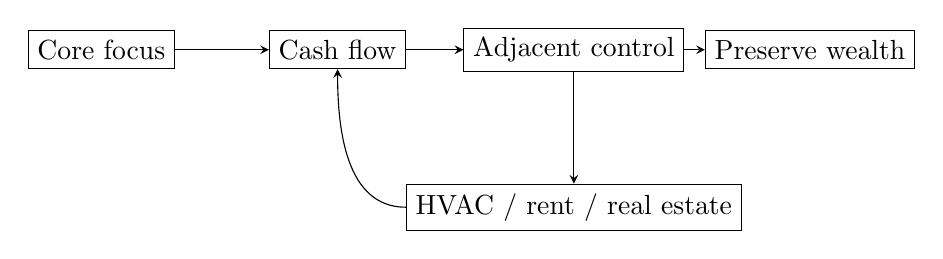
\begin{tikzpicture}[>=stealth]
\node[draw, rectangle] (a) at (0,0) {Core focus};
\node[draw, rectangle] (b) at (3,0) {Cash flow};
\node[draw, rectangle] (c) at (6,0) {Adjacent control};
\node[draw, rectangle] (d) at (9,0) {Preserve wealth};
\node[draw, rectangle] (e) at (6,-2) {HVAC / rent / real estate};

\draw[->] (a) -- (b);
\draw[->] (b) -- (c);
\draw[->] (c) -- (d);
\draw[->] (c) -- (e);
\draw[->] (e.west) to[out=180,in=-90] (b.south);
\end{tikzpicture}
\end{figure}

This diagram is not a reconstruction of a board drawing; it is an editorial compression of the lecture's mechanism. We begin with concentration. Concentration gives cash flow. Cash flow allows adjacent control. Adjacent control feeds margin back into the same system and turns diversification from distraction into preservation.

\section{Peace, Dry Powder, and the Tipping Point}

Before the lecture turns to its last executive interview, it inserts a short but important correction through Dante. The correction is philosophical: peace should be sought instead of financial gain, or at least prior to being ruled by financial gain. The host immediately restates the lesson: if we pursue money alone, we will not find peace and we will not find happiness. This matters structurally. Without it, the lecture would end as pure acquisition logic. With it, the lecture is forced to distinguish wealth from orientation.

From there the lecture returns to formal business reasoning through the final healthcare executive. Here the central object is liquidity. We are told to spend about half of what we make and to keep dry powder on the side for opportunities and requirements.

\begin{definition}
Dry powder is liquid cash held in reserve so that one can move when investments, people, ideas, or unexpected obligations appear.
\end{definition}

The lecture's policy can be written schematically as

\begin{equation}
E \approx \tfrac12 I,\qquad C_{\mathrm{dry}} = I - E > 0.
\end{equation}

Here \(I\) is annual income, \(E\) is annual spending, and \(C_{\mathrm{dry}}\) is the cash reserve. The point is not an exact personal-finance law. The point is that opportunity requires liquidity. If all capital is committed, there is nothing left with which to act.

The lecture then turns from liquidity to scaling. The final executive says that the hardest part of going from seven figures to eight and nine is building enough infrastructure to support the business: more people, more technology, more sales, more marketing, more commercialization. The end state is what he calls an industry utility, meaning a condition in which not using the product leaves one at a disadvantage.

We can preserve that scaling chain as

\begin{equation}
K_{\mathrm{scale}}
=
K_{\mathrm{people}}
+
K_{\mathrm{tech}}
+
K_{\mathrm{sales}}
+
K_{\mathrm{marketing}}
+
K_{\mathrm{comm}}
\longrightarrow
U_{\mathrm{industry}}.
\end{equation}

This is again not a measured growth equation. It is the lecture's causal order. One does not reach a tipping point by idea alone. One reaches it by assembling enough infrastructure that the product becomes difficult to ignore.

The last personal lesson of the lecture closes the circle. What most enabled the executive's rise was not a private trick but helping others succeed. One hires strong people, mentors them, pulls them up the ladder, and thereby stays near the top of the food chain. The lecture ends, then, where it had been drifting all along: away from isolated heroics and toward systems of people.

\section{Summary}

If we compress the lecture too hard, it becomes a list of millionaire quotes. If we preserve its order, it becomes a coherent progression. First we are shown wealth in the wild. Then we are told that scale depends on knowing the customer and treating people properly. Then we are told that the company is not the CEO, that athletes also require disciplined structures around them, that exits create reinvestment power, that teams build large outcomes, that delegation and equity separate ownership from labor, that concentration should precede diversification, that vertical integration internalizes margin, that peace must not be displaced by money, and that dry powder and infrastructure are what make later scale possible.

The mathematics here is light, but it is not empty. It consists of thresholds, splits, counts, reserves, and causal chains. That is exactly what this lecture offers: not abstract theory, but a sequence of explicit mechanisms by which money is earned, protected, multiplied, and made compatible with a larger human life.